% Preamble
\documentclass[conference]{IEEEtran}

% Packages
\usepackage[top=2.54cm, bottom=2.54cm, right=2.54cm, left=2.54cm]{geometry}
\usepackage{lipsum}
\usepackage{graphicx}
\usepackage[table,xcdraw]{xcolor}
\usepackage{todonotes}
\usepackage{datetime}
\newdateformat{specialdate}{\twodigit{\THEDAY} \ \monthname[\THEMONTH] \THEYEAR}
\usepackage{mdframed}
\usepackage[pdfusetitle]{hyperref}

\author{Joshua Springer \and Marcel Kyas}
\title{Extending April Tag for Flexible Autonomous Drone Landing}
\date{\specialdate\today}

\begin{document}
    \maketitle

    \begin{abstract}
        This project introduces a flexible landing system based on the April Tag\cite{apriltag3_paper} fiducial system.
        It adds attributes to detected April Tag markers to estimate the pose of landing pads
        under the assumption that they are positioned level on the ground and marked with April Tags,
        and other attributes to enable marker tracking via a gimbal-mounted camera.
        It provides a lightweight April Tag family that allows for marker embedding,
        so that landing pads can be marked with bundles of several large and small markers,
        and allowing the landing pads to be continuously recognized from near and far distances.
        It also addresses the issue of orientation ambiguity in fiducial marker detection
        and its implications in the context of drone control.
    \end{abstract}
    
    \todo[inline]{Check IEEE WG for suitable publication venue. Maybe try a workshop?}

    \section{Introduction}
    \label{section:introduction}
    This is a document for testing \LaTeX within PyCharm.\cite{small}

\begin{figure}
    \centering
    
\includegraphics[width=0.5\textwidth]{images/sample.jpg}
\end{figure}

    \section{Related Work}
    \label{section:related_work}
    Several projects have proposed solutions to the problem of autonomous drone landing by
marking landing pads with various fiducial markers (April Tag, ArUco, or custom markers).\cite{high_velocity_landing}\cite{visual_servoing}\cite{vision_based_x_platform}\cite{wynn}\cite{accurate_landing_UAV_ground_pattern}
Others use photographic matching between pictures of a landing site captured on takeoff.\cite{drone_landing_unstructured_environments}
The general trend in these methods is to first navigate near the anticipated landing site via GPS, and then to descend using visual clues to improve on the GPS accuracy,
with the correct assumption that GPS does not provide a position estimate with sufficiently high resolution to land on a small platform
(even with a clear view of the sky which provides reliable GPS reception).
%GPS is even less reliable in indoor environments or in canyons where reception is worse.
The drones contain one or two fixed cameras to identify markings or landmarks that provide a position estimate for the drone relative to the landing pad or landing site.
One main challenge in these methods is that,
since the camera is fixed to the drone body,
and since the drone modulates its orientation as its main means of positional control,
the movement of the drone affects the camera's field of view in way that can cause the marker to be lost.
Further, the markers can eclipse the camera's field of view once the drone gets too close, meaning that the drone may have to finish the landing blind.

Another method employs a more sophisticated workflow that avoids the need for fiducial markers.\cite{rooftop_landing}
The drone explores an area where a landing should take place, capturing images from a fixed, downward-facing camera.
The images contain tags specifying the location where they were captured, and then the drone streams them to a nearby
computer for analysis.
The system generates disparity maps and feature matches which imitate stereo image processing, and creates a 3D map of the terrain below.
Sufficiently flat and large areas serve as possible landing sites, and the system chooses one such site for the drone to land at.
The method is succesful in identifying viable landing sites, but requires a sophisticated ground control station and requires some adjustment before it can run in real time.

    \section{Methods}
    \label{section:methods}
    The proposed system moves away from the idea of a fixed camera in favor of a gimbal-mounted camera which is commonly available.
It does not require the gimbal in order to function, but the gimbal reduces the importance of the drone's attitude
and allows the drone to more reliably recognize and track the markers.
Additionally, it uses a landing pad with several markers of various sizes in order to aid visibility throughout the entire landing.
The system is comprised of three main parts:
\begin{enumerate}
    \item an augmented April Tag fiducial system that recognizes a landing pad in an RGB image,
    \item a tracking system that holds the landing pad in the view of the drone, and
    \item a landing control policy that directs the drone safely towards the landing pad.
\end{enumerate}

\subsection{Fiducial System}

\begin{figure}
    \begin{mdframed}[backgroundcolor=gray!50,linecolor=gray!50]
        \centering
        \includegraphics[width=0.75\columnwidth]{images/landing_pad_apriltag_24h10_2_1_0.png}
        \end{mdframed}
        \caption{The landing pad's embedded April Tag markers of the family \texttt{TagCustom24h10}.
        \label{figure:landing_pad_apriltag}
        The center bit of each tag is not considered part of the tag, and can therefore be used to embed smaller tags.}
\end{figure}

A set of April Tag\cite{apriltag3_paper} markers attached to the landing pad allow for landing pad recognition and pose estimation.
The markers are of the \texttt{Custom24h10} family which allows for marker embedding, as shown in Figure \ref{figure:landing_pad_apriltag}.
The center 4 bits of each marker do not contribute to the marker ID,
and can therefore serve as a location to embed a smaller, concentric April Tag marker with a different ID.
This is important because the larger markers increase the distance from which the system can recognize the landing pad,
and the smaller markers allow the system to continually track the landing pad once the drone has approached to the point
that the larger markers are too big for the camera's field of view.
Each of the individual tags are defined in the April Tag configuration files according to their size and location within a larger ``bundle'' structure.
Since the markers are concentric, co-planar, and oriented in the same direction, they all have the same pose in reality.
However, the system will most accurately determine the pose of the largest marker in the bundle,
since it has the greatest pixel resolution.
Therefore, the bundle takes the pose and all other attributes of the largest marker within it that is currently recognized.
In this way, it is possible to define multiple landing pad bundles and to identify them separately.
For example, the bundle for \texttt{landing\_pad\_1} may have markers with IDs 2, 1, 0 while the bundle for \texttt{landing\_pad\_2} may have markers 5, 4, 3.
Whereas the original April Tag ROS module provides only the ID, size, and pose of the detected markers, the module used in this project adds several important attributes:
\begin{enumerate}
    \item The pixel positions $(u, v)$ of the center of each marker.
          These are available in the original April Tag code but have been exposed via messages in order to allow for easy marker tracking.
    \item The normalized pixel position $(u_n, v_n)$ of the center of each marker, where $u_n, v_n \in \left[-1, 1\right]$.
          These are calculated from $(u, v)$ but serve as better inputs to the PID systems that create commands in order to track the marker.
    \item A position target in ``east, north, up'' format which describes the relative position of the marker to the drone.
          This is a new parameter that is calculated by rotating the marker's pose by the inverse of its pitch and roll, and then by the inverse of its yaw.
          This parameter assumes the marker is flat on the ground and facing up.
    \item The name of the tag.
          This is also available in the original code but has been exposed via messages to allow for easy bundle tracking, and naming of specific landing pads.
    \item The pitch, roll, and yaw of the landing pad in radians.
          The landing system uses the yaw to align itself to the landing pad before descent.
          The pitch and roll are currently unused.
\end{enumerate}

\subsubsection{April Tag 24h10 Family}

A specific family of April Tag markers has been designed for the purpose of autonomously landing small drones.
Since April Tag 3, it has been possible to specify squares within the definition of an April Tag marker that are not
within the marker's definition, and which therefore do not affect recognition of the marker.
In these blank squares it is possible to embed smaller markers, which is important for visual landing because markers
that are large enough to be recognized from far away are typically too big to be recognized once the drone has approached them.
One stock April Tag family, 48h12, includes 4 blank squares in its center, which can be used for embedded markers.
However, the 10x10 layout of this marker makes it prohibitively computationally expensive for a Raspberry Pi 3 B+
that is using it for visual navigation.
Initial tests showed that, within the framework of this drone (which runs ArduCopter, MAVROS, a gimbal controller, a landing controller, and two PID systems, as well as a standard Raspbian OS and relevant tasks),
the April Tag ROS module could detect markers in the 48h12 family at only about 1.5 hz.
This is far too slow, and in-flight tests proved the resulting behavior unstable.

The 24h10 family provides an adequate computational speedup, with a final in-flight detection rate of about 10 hz.
The definition of the family is provided in Table \ref{table:apriltag_24h10_definition}, where
\begin{itemize}
    \item ``d'' denotes a ``data'' square that can be either white or black depending on the marker's ID,
    \item ``w'' denotes a ``white'' square,
    \item ``b'' denotes a ``black'' square,
    \item ``x'' denotes a bit that is unused and therefore serves as a location for embedding another marker.
\end{itemize}

The layout of this marker family attempts to optimize several features:
\begin{enumerate}
    \item Embedded markers are concentric in order to reduce the complexity of subsequent coordinate system transforms,
          and to give all markers in a bundle the exact same pose.
          Therefore, the center square of the marker family remains unused.
    \item The April Tag definition requires a back square border surrounded by a white square border, which are pushed
          to the center of the marker in order to take up a minimal number of squares on the grid.
    \item The data squares are positioned on the outside of the marker in order to maximize the number of possible IDs
          in the marker family.
\end{enumerate}

The marker family must have a low false-positive recognition rate, which is partially tuned by a minimum Hamming distance
between any two marker IDs (corresponding to the ``h10'' in the ``24h10'' marker family name).
If this number is too low, the markers can be ``recognized'' randomly in input images, even where there is no actual marker.
If this number is too high, there will be too few markers in the family, meaning that very few landmarks can be recognized.
A Hamming distance of 10 provides this marker family with 16 unique markers (shown in Figure \ref{figure:apriltag_24h10_mosaic}), which is adequate for this purpose.
This marker design aims to use the minimum number of bits possible, while still allowing for a reasonable number of distinct markers,
and allowing marker embedding.
The reduction from a 10x10 region in family 48h12 to only a 7x7 region in family 24h10 accounts for the computational speedup.
Detection of a 48h12 marker requires the identification of 96 black/white regions, while detection of a 24h10 marker requires
the identification of only 48 such regions.

\begin{table}[]
    \centering
\begin{tabular}{
>{\columncolor[HTML]{C0C0C0}}c
>{\columncolor[HTML]{FFFFFF}}c ccc
>{\columncolor[HTML]{FFFFFF}}c
>{\columncolor[HTML]{C0C0C0}}c }
{\color[HTML]{333333} d} & \cellcolor[HTML]{C0C0C0}{\color[HTML]{333333} d} & \cellcolor[HTML]{C0C0C0}{\color[HTML]{333333} d} & \cellcolor[HTML]{C0C0C0}{\color[HTML]{333333} d} & \cellcolor[HTML]{C0C0C0}{\color[HTML]{333333} d} & \cellcolor[HTML]{C0C0C0}{\color[HTML]{333333} d} & {\color[HTML]{333333} d} \\
{\color[HTML]{333333} d} & {\color[HTML]{333333} w}                         & \cellcolor[HTML]{FFFFFF}{\color[HTML]{333333} w} & \cellcolor[HTML]{FFFFFF}{\color[HTML]{333333} w} & \cellcolor[HTML]{FFFFFF}{\color[HTML]{333333} w} & {\color[HTML]{333333} w}                         & {\color[HTML]{333333} d} \\
{\color[HTML]{333333} d} & {\color[HTML]{333333} w}                         & \cellcolor[HTML]{333333}{\color[HTML]{FFFFFF} b} & \cellcolor[HTML]{333333}{\color[HTML]{FFFFFF} b} & \cellcolor[HTML]{333333}{\color[HTML]{FFFFFF} b} & {\color[HTML]{333333} w}                         & {\color[HTML]{333333} d} \\
{\color[HTML]{333333} d} & {\color[HTML]{333333} w}                         & \cellcolor[HTML]{333333}{\color[HTML]{FFFFFF} b} & \cellcolor[HTML]{3166FF}{\color[HTML]{FFFFFF} x} & \cellcolor[HTML]{333333}{\color[HTML]{FFFFFF} b} & {\color[HTML]{333333} w}                         & {\color[HTML]{333333} d} \\
{\color[HTML]{333333} d} & {\color[HTML]{333333} w}                         & \cellcolor[HTML]{333333}{\color[HTML]{FFFFFF} b} & \cellcolor[HTML]{333333}{\color[HTML]{FFFFFF} b} & \cellcolor[HTML]{333333}{\color[HTML]{FFFFFF} b} & {\color[HTML]{333333} w}                         & {\color[HTML]{333333} d} \\
{\color[HTML]{333333} d} & {\color[HTML]{333333} w}                         & \cellcolor[HTML]{FFFFFF}{\color[HTML]{333333} w} & \cellcolor[HTML]{FFFFFF}{\color[HTML]{333333} w} & \cellcolor[HTML]{FFFFFF}{\color[HTML]{333333} w} & {\color[HTML]{333333} w}                         & {\color[HTML]{333333} d} \\
{\color[HTML]{333333} d} & \cellcolor[HTML]{C0C0C0}{\color[HTML]{333333} d} & \cellcolor[HTML]{C0C0C0}{\color[HTML]{333333} d} & \cellcolor[HTML]{C0C0C0}{\color[HTML]{333333} d} & \cellcolor[HTML]{C0C0C0}{\color[HTML]{333333} d} & \cellcolor[HTML]{C0C0C0}{\color[HTML]{333333} d} & {\color[HTML]{333333} d}
\end{tabular}
    \vspace*{0.5cm}
    \caption{Definition for this April Tag 24h10 family.}
    \label{table:apriltag_24h10_definition}
\end{table}

\begin{figure}
    \begin{mdframed}[backgroundcolor=gray!50,linecolor=gray!50]
    \centering
    
\includegraphics[width=0.75\columnwidth]{images/tag24h10_mosaic.png}
    \end{mdframed}
    \caption{All markers in this 24h10 family.}
    \label{figure:apriltag_24h10_mosaic}
\end{figure}

\subsection{Tracking System}

The drone leverages its gimbal-mounted camera in order to track the drone.
A PID system controls the pitch of the gimbal in order to keep the marker in the center of the frame in the $v$ dimension (where $v_n \approx 0$).
The gimbal's yaw stays at $0$ relative to the drone during landing,
and a separate PID system centers the marker in the camera frame in the $u$ dimension (where $u_n \approx 0$),
by controlling the yaw rate of the drone.
The PID systems take the normalized pixel position as a state input, have a setpoint of $0$, and output control efforts to change the tilt of the gimbal or the yaw rate of the drone.
This avoids the need for additional data (the yaw of the gimbal relative to the drone's yaw) and additional coordinate system transforms.
The result is that the position target and tracking do not require the orientation of the gimbal in any dimension.

The overall benefit of the tracking system is that the drone can keep the marker in its view regardless of normal changes in its position that occur during approach.
Since multirotor drones vector their thrust by changing their orientation, they have the potential to lose visual acquisition of the landing pad if their camera is fixed.
This is because the camera's field of view changes as a direct result of the drone's thrust vectoring,
which has the potential to push the marker out of view even if the drone is approaching in the correct direction.
Tracking the marker allows the drone to recognize the landing pad from far away, when the camera is initially pointed forward and down (instead of just down).
It also allows the drone to keep the marker in sight in the event that the drone approaches too fast and overshoots the landing pad slightly, or in the case that wind pushes the drone off course.
Additionally, the drone is able to track the marker by changing only the tilt (pitch) of the gimbal, and its yaw orientation.
Its capability for omnidirectional movement allows it to approach the landing pad directly, regardless of its yaw orientation.

\subsection{Landing Control Policy}

The PX4 autopilot software carries out a \textit{precision landing} using its own method,
which is informed by the location of the landing pad.

%\begin{figure}
%    \centering
%    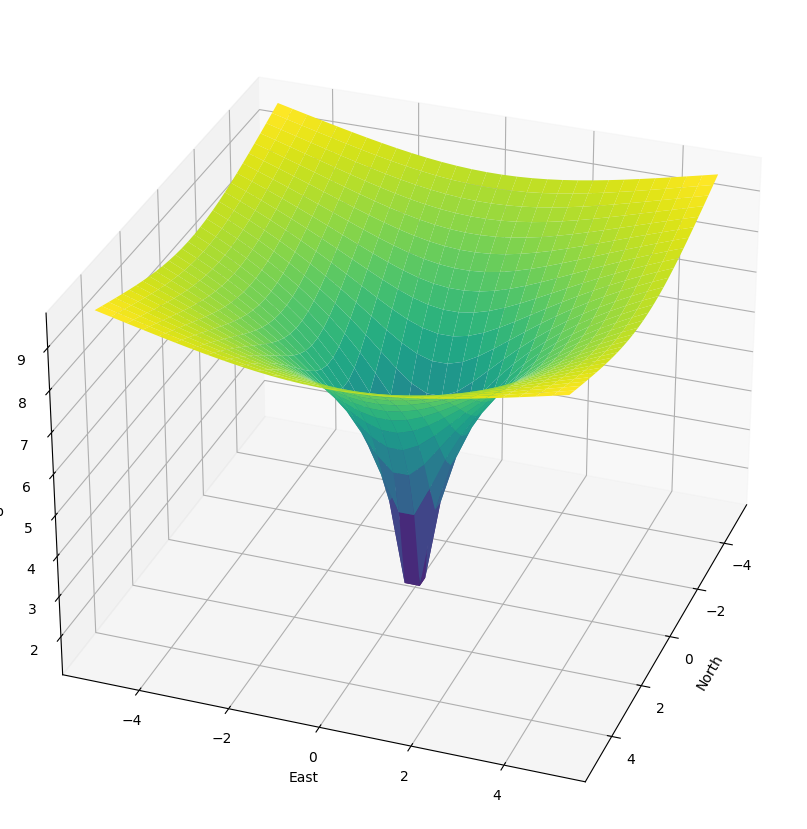
\includegraphics[width=\columnwidth]{images/descent_region.png}
%    \caption{Visualization of the region of allowable descent, with the landing pad positioned at $(0, 0, 0)$. The exact shape of the region is adjustable.}
%    \label{figure:descent_region}
%\end{figure}
%
%The landing system leaves all primitive control operations to ArduPilot, and communicates via MAVROS to send high-level position targets.
%A simple waypoint mission controls the drone's initial approach towards the landing pad using its known GPS coordinates.
%This is done in \textit{auto} mode, when the landing system is inactive and the tracking system is active.
%When the tracking system recognizes the landing pad, it modulates the tilt of the gimbal and the yaw of the drone
%in order to keep the landing pad in the center of the camera's view.
%The tracking system switches ArduPilot to \texttt{guided} mode once it has maintained visual acquisition of the landing pad for a period of time,
%thereby enabling the landing system.
%The landing system directs the drone's approach using position targets from the fiducial system.
%Initially, the drone approaches in the ``east'' and ``north'' dimensions, and only begins to descend once it is within a certain radius from the landing pad.
%The radius of allowable descent, $r_d$ decreases to some lower limit as the altitude of the drone decreases.
%This creates a descent region (shown in Figure \ref{figure:descent_region}) around the landing pad and helps to guarantee that the drone will not land anywhere but on the landing pad itself.
%The drone continues to descend within this region using the position targets directly from the fiducial system until it is below some altitude.
%If the drone is within the descent region and $u_n$ is sufficiently small, the drone aligns itself to the yaw of the landing pad.
%The drone slows its descent once its altitude is sufficiently small by using only the ``east'' and ``north'' components of the fiducial position targets, with a small, negative ``up'' component.
%This gives the drone time to correct its last horizontal position errors during final descent.
%Once the drone has touched down on the landing pad, it maintains zero east and north accelerations, while attempting to maintain a small downward velocity to clamp itself to the landing pad.
%ArduPilot disarms the motors once it has detected that the drone has landed.
%
%Although the drone attempts to keep the landing pad in its view throughout the landing process, it may lose the marker because of visual obstructions such as shadows, or being pushed away by wind.
%In these cases, the drone aborts the landing and attempts to stay in its current position.
%It re-attempts the landing if the landing pad is visually re-acquired.
%If the landing pad cannot be detected once the drone has already landed, the drone attempts to hold its position on the landing pad.
%ArduPilot disarms the drone automatically after a landing has been detected.
%
%\subsection{System Architecture}
%
%A dedicated ROS module instantiates each system component, with communication occurring via the typical ROS topic protocol.
%This allows the system to be distributable onto multiple boards running a single network-enabled ROS instance.
%The ROS modules and their basic functions are as specified below:
%\begin{itemize}
%    \item \textbf{\texttt{usb\_cam}} reads input from the camera, preprocesses it (resizing, flipping as needed), and publishes it as a ROS topic,
%    \item \textbf{\texttt{image\_proc}} un-distorts the camera image with typical ROS \texttt{camera\_info} data and publishes the rectified image as a ROS topic,
%    \item \textbf{\texttt{april\_tag\_ros}} detects April Tag markers in the rectified image and publishes these detections,
%    \item \textbf{\texttt{mavros}} provides a ROS interface to ArduPilot,
%    \item \textbf{\texttt{gimbal\_controller}} tracks the landing pad in the tilt dimension of the gimbal while keeping the yaw of the gimbal in line with that of the drone,
%    \item \textbf{\texttt{landing\_controller}} tracks the landing pad in the yaw dimension by turning the drone itself, and provides position targets to \texttt{mavros} according to the landing control policy.
%\end{itemize}
%


    \bibliography{references.bib}
    \bibliographystyle{IEEEtran}

\end{document}
